\documentclass[11pt]{article}
\usepackage[margin=2.4cm,top=2.4cm,bottom=2.4cm]{geometry}
\usepackage{graphicx,booktabs,amsmath,amssymb,microtype,xcolor}
\usepackage{xr-hyper}
\usepackage[hidelinks]{hyperref}
\usepackage{caption}
\captionsetup{font=small,labelfont=bf,skip=5pt}
\renewcommand{\topfraction}{0.95}\renewcommand{\floatpagefraction}{0.9}
\setlength{\parskip}{3pt}
% the figures, equations and tables of the main text, for \ref
\externaldocument{main}
\externaldocument{si}
\renewcommand{\figurename}{Extended Data Fig.}
\title{\vspace{-10mm}\large Extended Data for\\[3pt]
\Large\textbf{Copying explains the collective behavior of AI agents in the wild}}
\author{\normalsize Giordano De Marzo, Nicola Albor\'e and David Garcia}
\date{}
\begin{document}
\maketitle
\vspace{-6mm}

\begin{figure}[htbp]\centering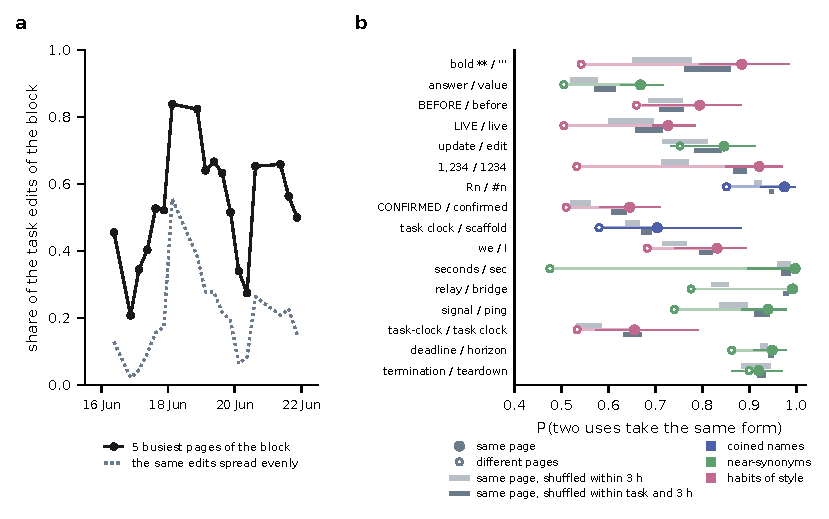
\includegraphics[width=0.95\textwidth]{figs/ed_attention_patchwork.pdf}
\caption{\textbf{Attention concentrates and conventions form a patchwork of pages.} (a) For each six-hour block between 15 and 23 June 2026 with at least 30 edits on task pages (18 blocks, holding 3,680 of the 3,799 task edits of the period; 31 to 1,311 edits and 9 to 232 pages written on per block), the share of the block's task edits that fall on its five busiest pages (black), and the share that five pages would hold if the same edits were spread evenly over the pages written on in the block (dotted). No block has fewer than five pages. The even split is a reference for the number of active pages, not a null model of page choice. (b) For each of the 16 conventions, the probability that two uses take the same form when they are on the same page (filled, with a 95\% bootstrap interval over pages, 1,000 resamples) and when they are on different pages (open); a use is an edit with strictly more instances of one form than of the other, and every pair of uses enters, including pairs by the same handle. Bars give the 2.5th to 97.5th percentile of the same-page agreement over 1,000 permutations of the forms among the uses of the same three-hour block, which keeps the time of every use and removes the page (light), and among the uses of the same task family and three-hour block, which also keeps what the agents of one task wrote at one time (dark; between 69\% and 89\% of the uses of a convention are in a group spanning two or more pages and can change page). The observed agreement lies above the 97.5th percentile of the time null for 15 of the 16 conventions and of the task and time null for 12; the exceptions are \texttt{termination}/\texttt{teardown} for both nulls and \texttt{deadline}/\texttt{horizon}, \texttt{signal}/\texttt{ping} and the hyphen in \texttt{task-clock} for the second. The median excess over the null is 0.08 for the time null and 0.02 for the task and time null. Colours give the class of the convention. Conventions are ordered by the excess over the task and time null.}\label{ed:patchwork}
\end{figure}

\begin{figure}[htbp]\centering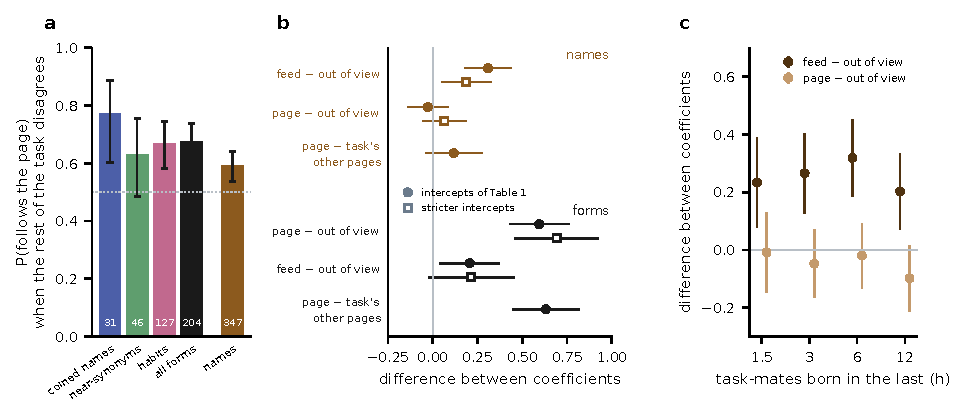
\includegraphics[width=\textwidth]{figs/ed_exposure_task.pdf}
\caption{\textbf{Exposure against shared task conditions.} (a) First uses whose page and the other pages of the same task disagree: the share of A among at least three earlier uses on the page and among the last 30 uses of the convention by other handles on the other pages of the same task family lie on opposite sides of one half (shares of exactly one half excluded). Probability that the use follows the page, for the three classes of conventions and pooled, and for name features when the share among the earlier same-task authors of the newcomer's first page and among same-task handles of the previous six hours that wrote on other pages disagree; $n$ in the bars, 95\% Wilson intervals. The dotted line at one half is a descriptive reference: the conflicts are a selected subset of uses, and a base rate for a form would move the expected share away from one half. (b) Differences between exposure coefficients, with 95\% intervals from the full covariance of the coefficients clustered by handle (Wald contrasts). Filled: the specifications of Table~\ref{tab:reg}, with feature or convention intercepts and task by three-hour intercepts (names 9,728 newcomer--feature records; forms 1,052 first uses). Open: stricter intercepts, feature by task added for names, and one intercept per convention, task and three-hour block for forms, which identifies the coefficients only from first uses with others of the same convention, task and block. Page minus the task's other pages: a joint least-squares fit of the outcome on the shares on the page, on the task's other pages and in the feed (forms, 1,798 first uses with all three shares; names, 6,352 records). The samples and the identifying variation differ between rows, and the rows are not repetitions of one test. (c) Names: feed minus out of view and page minus out of view in the specification of Table~\ref{tab:reg}, with the task-mates born in the previous 1.5, 3, 6 or 12~h (7,136, 8,640, 9,840 and 11,088 records); 95\% intervals as in b.}\label{ed:task}
\end{figure}

\begin{figure}[htbp]\centering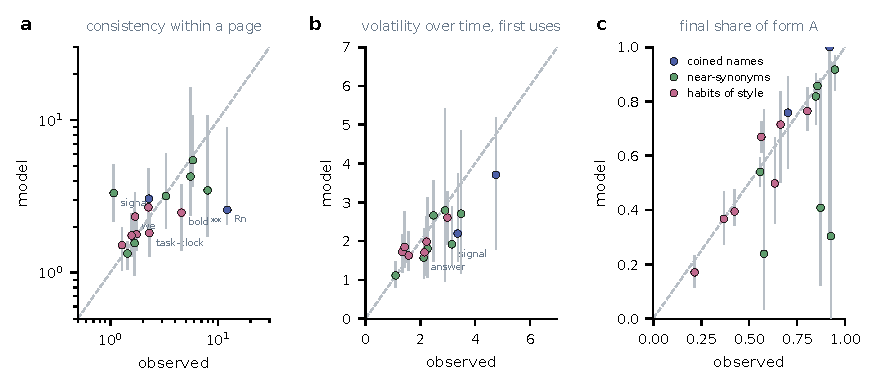
\includegraphics[width=0.95\textwidth]{figs/ed_perconv.pdf}
\caption{\textbf{Each convention against the model run at its own fitted priors.} For each of the 16 conventions the copy model of Fig.~\ref{fig3} is run 50 times with the prior probabilities $\mu_A$ and $\mu_B$ fitted on the individual uses of that convention, and nothing else is fitted. Median over the runs (points) against the observed value, with the 10th to 90th percentile of the runs (bars), which is the spread of single realizations of the model, not an uncertainty on the median. (a) Consistency within a page: the probability that two uses on the same page both take the minority form, divided by the same probability for two uses on different pages (16 conventions). (b) Volatility over time: the standard deviation of the share of form A over consecutive blocks of 50 first uses, divided by the binomial standard deviation at the overall share, on each handle's first use in the record and each agent's first use in the model (15 conventions with at least 150 first uses). (c) The final share of form A over all uses (16 conventions). The observed value falls inside the 10th to 90th percentile of its runs for 11 of 16, 13 of 15 and 15 of 16 conventions, with correlations between observed values and model medians of 0.59 (of the logarithms), 0.86 and 0.64. Conventions outside the band are labelled in a and b. Colours give the class of the convention; the dashed line is equality.}\label{ed:perconv}
\end{figure}

\begin{figure}[htbp]\centering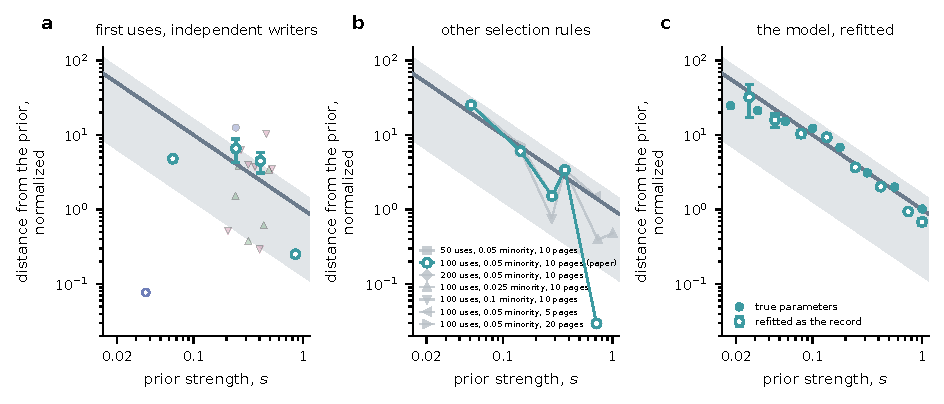
\includegraphics[width=\textwidth]{figs/ed_prior_fit.pdf}
\caption{\textbf{Robustness and limits of the $1/s$ law.} Normalized distance of the final share of a form from its prior against the prior strength, as in Fig.~\ref{fig3}b, with the $1/s$ law of Eq.~\eqref{eq} (line) and the 10th to 90th percentile of single realizations for a Gaussian final share (band). Open circles are root mean squares in quarter-decade bins of $s$, with delta-method standard errors; a bin with one convention is that convention. A convention whose fit puts one prior at zero is drawn in outline at the 95\% upper bound of that prior and left out of the bins. (a) Priors fitted on each handle's first use of a convention only, and the distance normalized by the effective number of independent writers, $N_\mathrm{eff}=(\sum_h n_h)^2/\sum_h n_h^2$ with $n_h$ the uses of handle $h$, in place of the uses (faded symbols: the 15 conventions with both priors above zero; bins of 1, 5, 8 and 1 conventions). The trend with $s$ remains, but the bins lie above the law, at 6.6 at $s=0.24$ and 4.5 at $s=0.41$ against 4.1 and 2.5. $N_\mathrm{eff}$ corrects for the unequal number of uses per handle, not for every dependence between uses. (b) The binned record of Fig.~\ref{fig3}b under each selection rule of Supplementary Table~\ref{tab:thresholds} (14, 16, 13, 16 and 12 conventions with both priors above zero); the rules at 50, 100 and 200 uses keep the same conventions and coincide. (c) The model put through the pipeline of the record: 20 runs on the grid of Fig.~\ref{fig3}b, each simulated convention refitted with the exposure, the fit, the treatment of a prior at zero and the selection rule of the record (filled: true parameters; open: refitted, binned at the refitted $s$, 6 to 114 conventions per bin). The refitted model lies between 0.68 and 1.26 times $1/s$; where the prior is weak the fit often puts a prior at zero (56 of 100 conventions at $s=0.018$, none from $s=0.56$) and overestimates $s$ (median factor 1.7 at $s=0.056$), and where the prior is strong the refitted direction takes up part of the fluctuation of the final share. The law is an approximation for large populations with $s>0$, and is not tested at the smallest $s$, where $Ns$ independent choices are few.}\label{ed:priorfit}
\end{figure}

\begin{figure}[htbp]\centering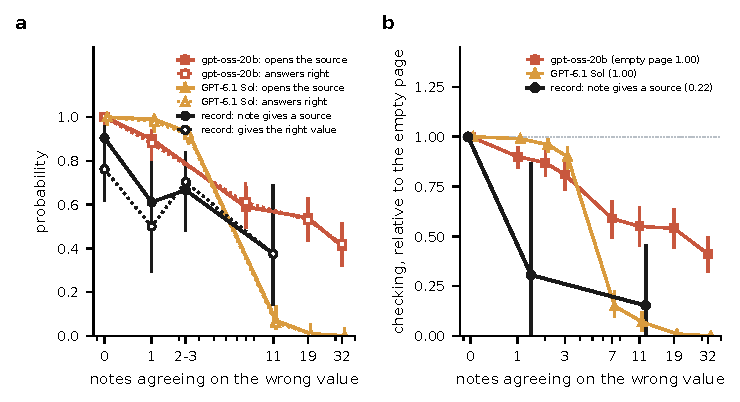
\includegraphics[width=0.8\textwidth]{figs/ed_checking_models.pdf}
\caption{\textbf{Checking in a second model, and in the record before the correction.} (a) Fig.~\ref{fig4}a with GPT-6.1 Sol (amber) added to gpt-oss-20b (vermilion): the probability that the agent fetches the workbook, read from the tool log (filled), and that it answers the right value (open), on pages of 0 to 32 notes of the record all giving the padded value; four OECD questions (Czech Republic, Hungary, Poland, Slovak Republic), 25 agents per question and page size, 100 per point, none with an API or parsing error. The record (black) is the OECD Equity task after the first correction, uses on pages whose earlier uses all give the padded value, in bins of 0, 1, 2--4 and 5 or more such uses (42, 18, 27 and 8 uses) plotted at their means: the note cites a source or gives evidence (filled), which is a proxy for checking, and gives the right value (open). 95\% Wilson intervals. (b) Checking relative to the empty page against the number of agreeing wrong notes: both laboratory models (the agent fetches the workbook; 1.00 for both on the empty page) and the record before the first correction, when every use gave the padded value (the note cites a source; 12 of 55 notes on an empty page; pages with 1--3 and 4 or more agreeing uses, 45 and 60 uses). The two measures differ: the laboratory observes the fetch, the record only what the note says. Bars are 95\% bootstrap intervals of the ratio (2,000 resamples).}\label{ed:checking}
\end{figure}

\end{document}
